% !TeX spellcheck = en_US
\section{Phospholipids}
\label{section:metodeLipide}

\subsection{Preparation of lipid coated slides}

To create the slides with parylene and lipids, a cover glass (\SI{5}{\milli\meter} diameter) is used as base. the cover glass is coated with a thin layer of parylene. The coated cover glass is dipped into lipid solution. The cover glass is dried, leaving behind a lipid layer. The prepared slides are then used in plunge freezing.

Two different kind of lipids are used: DOPC and EGG-PC. DOPC is storaged as a powder. The DOPC powder is solved in Ethanol ($25\,\si{\milli\gram}/1\,\si{\milli\liter}$ lipid to solvent) for application. 
EGG-PC is shipped solved in chloroform in two different ratios: $25\,\si{\milli\gram}/1\,\si{\milli\liter}$ and $10\,\si{\milli\gram}/1\,\si{\milli\liter}$. The solution is shipped in vials.

The lipid solution is transferred into several small bottles. small bottles are chosen because solution forms a lubrication film on the thread of the lid. this prevents the lid from closing airtight. This leads to evaporation of the solvent over time, making the bottle unusable. In the coating process, solution often drops onto the threads, making a bottle only usable in one coating session. By splitting the solution into multiple flask, more slides can be covered from one batch of solution.

\section{Solubility lipids}

In the previous chapter, the method of using a sacrificial layer to detach ice is discussed. For this, lipids need to be solved at cryogenic temperatures. As not every lipid is dissoluble in all solvents, an experiment is conducted to obtain solvents at room temperature. Then the best solvents are tested at cryogenic temperatures.

Tests are conducted to find a solvent to dissolve a sacrificial layer out of lipids. Two consecutive solubility experiments are proposed. The first experiment is conducted at room temperature. the aim is to find solvents with high solubility at room temperature. the candidates with high solubility are then tested in the next experiment at cryogenic temperature. the aim is now to find solvents with also high solubility at cryogenic temperatures. The first experiment is conducted as there are only three baths available at cryogenic temperature. therefore the throughput for experiments is limited.

\subsubsection{at room temperature}

The Solvent are chosen based on availability, freezing point and safety. The solvents are all readily available in the laboratory. Some were ordered before the test. Also all chosen solvent are save to use in a well ventilated room. The followup experiment cannot be conducted under a extractor hood as too much space is taken up with the experiment. Also the solvent or solvent mixture needs to stay liquid at around \SI{-140}{\degreeCelsius} to assure that the ice layer on top stays vitrified. The tested substances are 4-Methyl Pentene, 3-Methyl Pentene, 1-Pentene, Isopentane, 1-Propanol, Pentane and Ethanol. 

Each solvent is put in a separate bottle. The lipid coated slides are prepared as previously described. For each solvent, a slide is put in the corresponding bottle. After \SI{15}{\minute}, the slides are removed and examined. The results are documented in a list. When all streaks caused by the lipid layer disappeared, the solvent is tested in the next experiment.

The solubility of lipids at room temperature in different solvents are determined. For this experiment the cover glasses are coated with lipids. Then a first reference image was taken. Then the cover glass is given into a small container with the potential solvent. After 15 minutes, the cover glass is removed and compared under the microscope with the reference picture. If streaks created from lipids are still as visible as before, the lipids are categorized as insoluble in this solvent. If the streaks partially dissapeared and/or are less visible, the lipids are categorized as partially soluble in this solvent. Last if the streaks completely disappear, the lipids are assinged as soluble in the solvent (Table \ref{table:LoeslichkeitRaumtemperatur}).

\begin{figure}[hbt!]
	\centering
	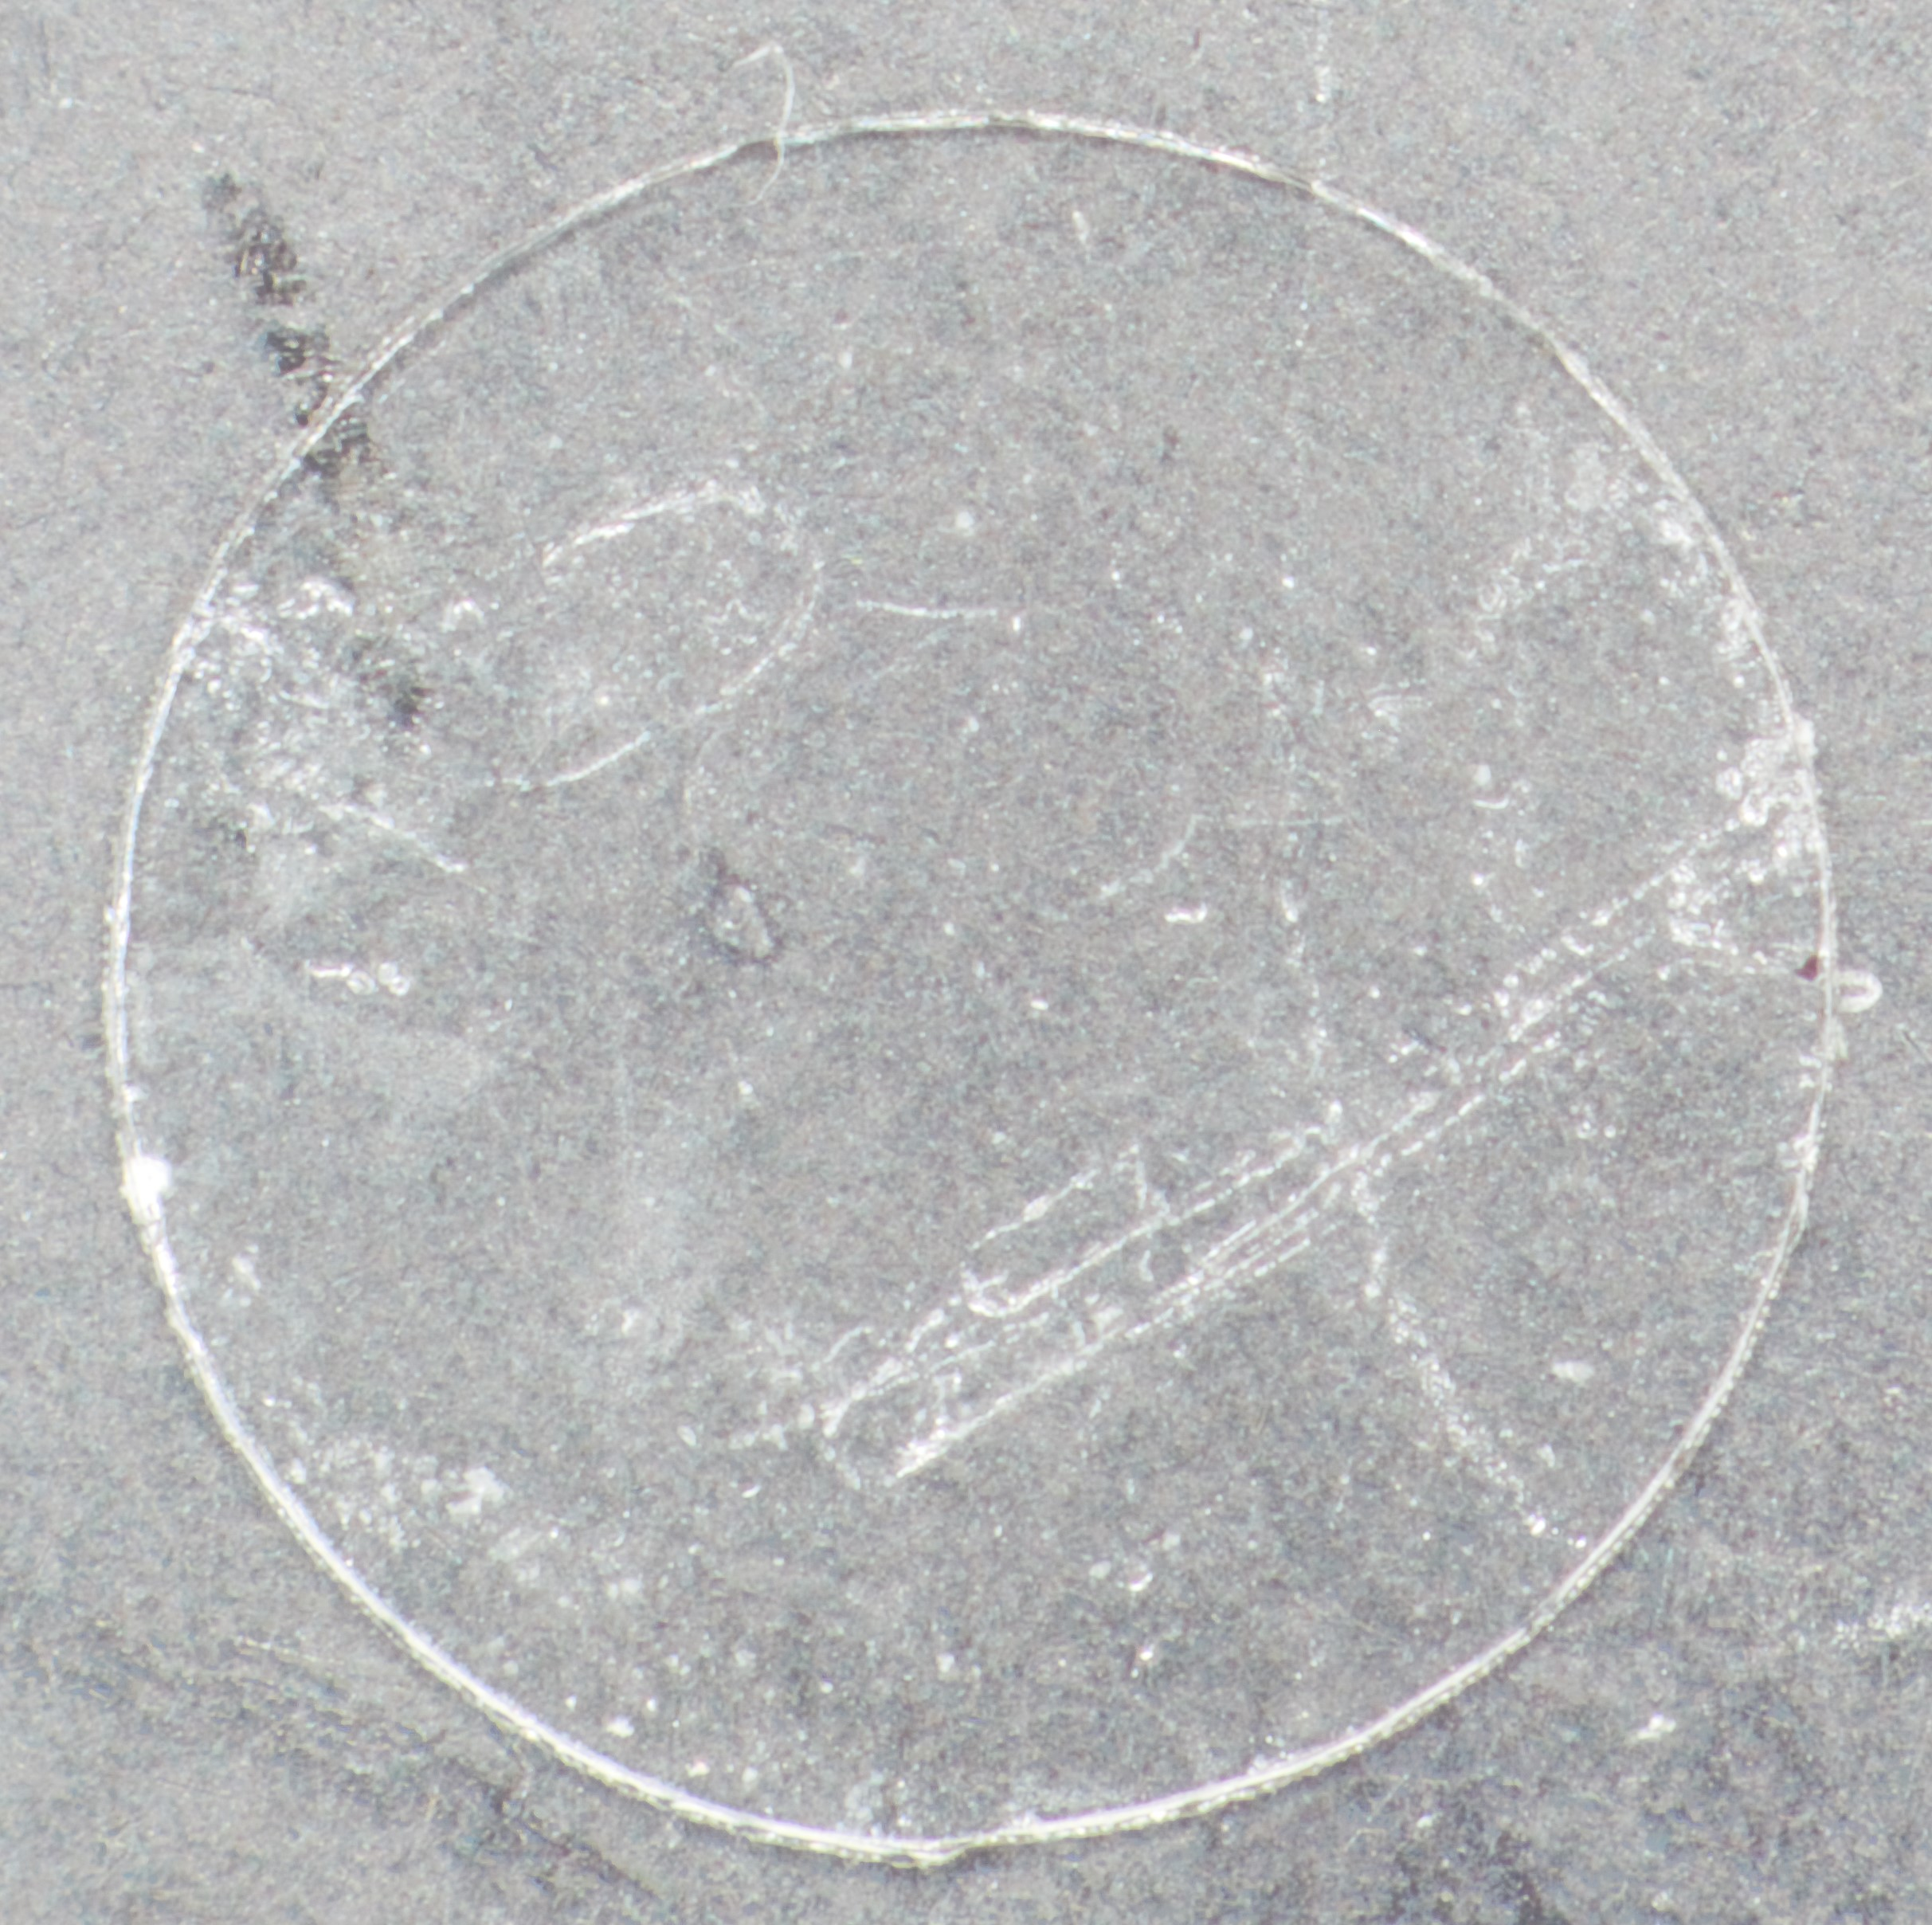
\includegraphics[width=7cm]{SlideWIthLipidStreaks.jpg}
	\caption{Example of a $\varnothing$\SI{5}{\milli\meter} cover glass with lipid residuals on the surface.}
\end{figure}


\begin{table}[hbt!]
	\centering
	\begin{tabular}{|l|c|c|}
		\hline
		potential solvent & solubility EGG-PC & solubility DOPC \\
		\hline
		\hline
		4-Methyl Pentene & soluble & N/A  \\ 
		\hline
		3-Methyl Pentene & slightly soluble & insoluble \\
		\hline
		1-Pentene & insoluble & insoluble \\
		\hline
		Isopentane & soluble & slightly soluble\\
		\hline
		1-Propanol & soluble & soluble\\
		\hline
		Pentane & soluble & insoluble\\
		\hline
		Ethanol & N/A & soluble\\
		\hline
	\end{tabular}
	\caption{Result of solubility tests at room temperature. Soluble indicates solvents which are able to visibly solve all lipids off a cover glass. slightly soluble indicates solutions which are able to solve lipids with residuals. Insoluble indicates no visible removal of tested lipid.}
	\label{table:LoeslichkeitRaumtemperatur}
\end{table}



\subsubsection{at cryogenic temperature}
\label{chapter:meltingtemp}

Solubility is temperature dependent. The process of dissolving a solute in a solvent can be broken up in three parts: First, the structure of the solute must be broken up with energy. Second the structure of the solvent is broken up alos taking energy. Last, the solute and solvent are rearranged into a new structure which releases energy. Depending on the ratio of energy taking up by breaking the structure of solute and solvent and energy released at rearranging, the process is endo- or exothermic \cite{ZafirJaveed.}. Exothermic processes have higher solubility at low temperatures, while Endothermic processes habe higher solubility at high temperatures \cite{Mortimer.2007}. Therefore, solubility needs to be tested at the same temperature as in application.

A quick look at the chemical structure of lipids reveals that solving lipids is most likely endothermic. lipids ordered in layers are held together with van-der-vaals forces, hydrogen bondings and electrostatic bonds \cite{RWayneAlbers.1999}. This results in a very strong bond between lipids. Therefore, a high amount of energy is needed to break up the lipid layer structure. This makes a resulting endothermic dissolving process likely.

The experiment is conducted at \SI{-140}{\degreeCelsius}. The solvents are given in liquid nitrogen cooled baths, which are regulated to the desired temperature. A slide is given into the cold solvent for \SI{15}{\minute}. Then the slide is examined for leftover streaks as before.

The freezing point of tested solvents are not all below \SI{-140}{\degreeCelsius}] (Table \ref{table:SchmelztemperaturLösungsmittel}). Still, solvents with a high freezing point can be mixed with other solvents with lower freezing point to lower the freezing point of the mixture. Alternatively, the temperature can be raised over the freezing point, but this could risk the ice to loose the vitrified state.

\begin{table}[hbt!]
	\centering
	\begin{tabular}{|l|c|}
		\hline
		solvent & melting point in °C \\
		\hline
		\hline
		4-Methyl Pentene & -154 \\ 
		\hline
		3-Methyl Pentene & -154 \\
		\hline
		1-Pentene & -165 \\
		\hline
		Isopentane & -160 \\
		\hline
		1-Propanol & -126 \\
		\hline
		Pentane & -129 \\
		\hline
		Ethanol & -114 \\
		\hline
	\end{tabular}
	\caption{Melting Point in °C for tested solvents.}
	\label{table:SchmelztemperaturLösungsmittel}
\end{table}

This experiment shows that each three different solvent exist for EGG-PC and DOPC with high solubility (Table \ref{table:LoeslichkeitRaumtemperatur}). Following these results, solvents categorized with "soluble" are tested regarding solubility at temperatures of \SI{-140}{\degreeCelsius}. As not all solutions are liquid at \SI{-140}{\degreeCelsius} (Table \ref{table:SchmelztemperaturLösungsmittel}), they are tested at higher temperatures above their melting point, as mentioned in chapter \ref{chapter:meltingtemp}. In addition they are tested as mixtures with other solvents with a lower melting point. Additionally liquid ethane is tested as solvent. Ethane was not tested at room temperature, as the boiling point is at \SI{-88.6}{\degreeCelsius} \cite{PubChem.29.08.2023}.

In the experiment, no tested solvent was able to completely solve lipids at \SI{-140}{\degreeCelsius} and within \SI{15}{\minute} (Table \ref{table:Cryoloeslichkeit}). Also streaks of applied lipids did not only stay partially behind, but also new streaks appear on the glass slides. This means that some lipids redistributed on the same glass slide.

Using solvents to remove a sacrificial layer, a high solubility is required. In practice, the sacrificial layer is completely covered by the ice layer except the edges. Therefore area of contact with the solvent is small, slowing the process considerably. Additionally, as the ice layer needs to stay vitrified. The temperature cannot be raised over \SI{-140}{\degreeCelsius} to speed up the process.

The solving process of lipids proves to be endothermic. This means that heat is needed to solve lipids, so cold temperature heavily decrease solubility. This effect was observed over the last experiments by all solvents to varying degree. It can be assumed that the majority of solvent lipids mixtures are endothermic which is very disadvantageous for finding a potential solvent lipid candidate. Strongly exothermic solvents could heat up the ice enough to crystallize the ice. So weakly exothermic solvents would be optimal for this task.


\begin{table}[hbt!]
	\begin{subtable}{\linewidth}
		\centering
		\begin{tabular}{|l|l|}
			\hline
			Solvent & Result \\
			\hline
			\hline
			Pentane & soluble at \SI{-125}{\degreeCelsius} \\
			\hline
			4-methyl pentene & insoluble \\
			\hline
			\makecell[l]{1:1 volume ratio\\ HFE to 1-Propanol} & \makecell[l]{not mixable,\\ slightly soluble}\\
			\hline
			Liquid ethane & insoluble\\
			\hline
		\end{tabular}
		\caption{EGG-PC}
		\label{table:EGG-PCCryoloeslichkeit}
	\end{subtable}
	\begin{subtable}{\linewidth}
		\centering
		\begin{tabular}{|l|l|}
			\hline
			Solvent & Result \\
			\hline
			\hline
			\makecell[l]{1:4 volume ratio\\ 1:2 molar ratio\\ Ethanol to Isopentane} & slightly soluble\\
			\hline
			\makecell[l]{1:2 volume ratio\\ 1:1 molar ratio\\ 1-Propanol to Isopentane} & insoluble \\
			\hline
			Isopentane & slightly soluble\\
			\hline
			1-Propanol & \makecell[l]{at \SI{-130}{\degreeCelsius}\\ slightly soluble}\\
			\hline
			Liquid ethane & insoluble \\
			\hline
		\end{tabular}
		\caption{DOPC}
		\label{table:DOPCCryoloeslichkeit}
	\end{subtable}
	\caption{ in \ref{table:EGG-PCCryoloeslichkeit} for EGG-PC, no sufficient solubility at -140°C was found. In \ref{table:EGG-PCCryoloeslichkeit}, DOPC was tested but also no proper solution was found.}
	\label{table:Cryoloeslichkeit}
\end{table}

Additionally, some solvents tested are soluble in water. It is unknown whether the solvents could be solved or diffuse inside the ice layer at \SI{-140}{\degreeCelsius}. Therefore the ice layer could be changed in some undesired manner. if a sufficient solvent is found and the solvent is soluble in water, a potential change of the vitrified ice needs to be addressed.
